\documentclass[10pt]{article}
\usepackage[margin=0.6in]{geometry}
\usepackage{booktabs}
\usepackage{graphicx}
\usepackage{pgfplots}
\usepackage{xcolor}

\pgfplotsset{compat=1.18}

\definecolor{baselineblue}{RGB}{76,114,176}
\definecolor{exporange}{RGB}{221,132,82}

\begin{document}

\begin{center}
{\Large FlashOCC Baseline vs. R50 + Focal Loss (Continued Training)}

\vspace{0.2em}
\normalsize Occ3D-nuScenes validation set, 6019 samples
\end{center}

\begin{center}
\scriptsize
\setlength{\tabcolsep}{7pt}
\resizebox{\textwidth}{!}{%
\begin{tabular}{lccc}
\toprule
Class & FlashOCC (Baseline) & R50 + Focal Loss (Continued) & $\Delta$ \\
\midrule
others & 6.13 & 6.88 & \textbf{+0.75} \\
barrier & 34.62 & 38.89 & \textbf{+4.27} \\
bicycle & 10.17 & 11.66 & \textbf{+1.49} \\
bus & 38.18 & 40.19 & \textbf{+2.01} \\
car & 41.48 & 45.26 & \textbf{+3.78} \\
construction\_vehicle & 14.28 & 17.00 & \textbf{+2.72} \\
motorcycle & 14.07 & 16.66 & \textbf{+2.59} \\
pedestrian & 14.73 & 19.28 & \textbf{+4.55} \\
traffic\_cone & 13.38 & 16.13 & \textbf{+2.75} \\
trailer & 26.68 & 28.68 & \textbf{+2.00} \\
truck & 29.85 & 32.57 & \textbf{+2.72} \\
driveable\_surface & 76.89 & 78.66 & \textbf{+1.77} \\
other\_flat & 34.87 & 38.28 & \textbf{+3.41} \\
sidewalk & 46.86 & 48.42 & \textbf{+1.56} \\
terrain & 51.73 & 51.87 & \textbf{+0.14} \\
manmade & 37.08 & 37.73 & \textbf{+0.65} \\
vegetation & 32.04 & 32.71 & \textbf{+0.67} \\
free & -- & 87.40 & -- \\
\midrule
\textbf{Overall mIoU} & \textbf{30.77} & \textbf{32.99} & \textbf{+2.22} \\
\bottomrule
\end{tabular}%
}
\end{center}

\vspace{0.6em}

\begin{center}
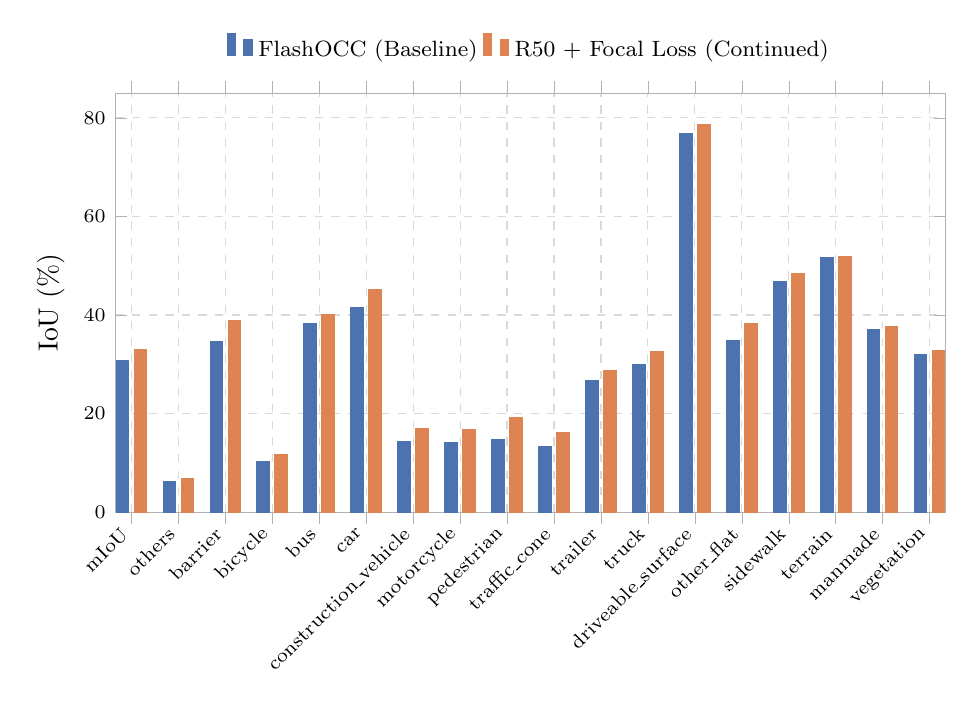
\begin{tikzpicture}
\begin{axis}[
    ybar,
    width=\textwidth,
    height=6.9cm,
    bar width=4.5pt,
    ymin=0,
    ymax=85,
    ylabel={IoU (\%)},
    symbolic x coords={
        mIoU,others,barrier,bicycle,bus,car,construction\_vehicle,motorcycle,
        pedestrian,traffic\_cone,trailer,truck,driveable\_surface,other\_flat,
        sidewalk,terrain,manmade,vegetation
    },
    xtick=data,
    xticklabel style={rotate=45, anchor=east, font=\scriptsize},
    yticklabel style={font=\scriptsize},
    legend style={
        at={(0.5,1.05)},
        anchor=south,
        legend columns=2,
        draw=none,
        font=\footnotesize
    },
    grid=major,
    grid style={dashed, gray!30},
    axis line style={gray!60},
    tick style={gray!60},
    enlarge x limits=0.02
]
\addplot[fill=baselineblue, draw=baselineblue] coordinates {
    (mIoU,30.77)
    (others,6.13)
    (barrier,34.62)
    (bicycle,10.17)
    (bus,38.18)
    (car,41.48)
    (construction\_vehicle,14.28)
    (motorcycle,14.07)
    (pedestrian,14.73)
    (traffic\_cone,13.38)
    (trailer,26.68)
    (truck,29.85)
    (driveable\_surface,76.89)
    (other\_flat,34.87)
    (sidewalk,46.86)
    (terrain,51.73)
    (manmade,37.08)
    (vegetation,32.04)
};
\addplot[fill=exporange, draw=exporange] coordinates {
    (mIoU,32.99)
    (others,6.88)
    (barrier,38.89)
    (bicycle,11.66)
    (bus,40.19)
    (car,45.26)
    (construction\_vehicle,17.00)
    (motorcycle,16.66)
    (pedestrian,19.28)
    (traffic\_cone,16.13)
    (trailer,28.68)
    (truck,32.57)
    (driveable\_surface,78.66)
    (other\_flat,38.28)
    (sidewalk,48.42)
    (terrain,51.87)
    (manmade,37.73)
    (vegetation,32.71)
};
\legend{FlashOCC (Baseline), R50 + Focal Loss (Continued)}
\end{axis}
\end{tikzpicture}
\end{center}

\noindent\textbf{Figure 1.} Grouped bar chart comparing the baseline with the R50 + Focal Loss continued-training experiment. The ``free'' score is listed in the table but omitted from the chart because the baseline value is unavailable and it is not part of mIoU.

\end{document}
